\chapter[2021 June]{June 2021}

\section[2021/06/11]{Friday, 11 June 2021}

\subsection{Centroid Detection for Multiple Cubes}

Previous results have shown that segmentation of the top face of the cube based on light intensity offers the most promising avenue to robustly detect and localise the cube. In order to develop this concept further, several adjustments were made to the previous image processing test setups. Firstly, it was previously demonstrated that the introduction of colour information into the image through the addition of a coloured background offers no better performance than pure light intensity information. Therefore, in order to maximise the light intensity differential between the reflective top face of the cube, a plain matte black paper background was introduced. Secondly, it was observed that when the angle between the light incident on the top face of the cube and the light reflected into the camera is minimised, the light intensity on the top face of the cube as observed by the camera is maximised. To make the most of this effect, the camera was placed parallel to the base plane at a height of approximately 500 mm with two bright \ac{LED} lights on either side angled toward the centre of the base plane. Lastly, to test that the ability of the image processing algorithm to detect multiple cubes in the same image with variying top face light intensities, multiple cubes were placed randomly on the base plane.

\FigRef{fig:multiple-cubes} shows the image that was captured with the above setup. Note the light intensity on the top face of each cube. The first step in extracting the contours from the image is to apply binary thresholding to the image to segment the top faces of the cubes. In preparation for this, the image was first converted to grayscale and blurred. The binary threshold in which only pixels with intensities greater than 140 out of 255 were retained. This resulted in a well segmented collection of cube top faces. The OpenCV contour detection algorithm was then applied to this binary images which resulted in the red contours shown in \FigRef{fig:multiple-cube-centroids}. Finally, the moment of each contour was calculated and used to find the centroid of each face. These centroids are indicated as blue dots in \FigRef{fig:multiple-cube-centroids}. All the cube centroids were successfully detected in terms of the image coordinate system which is sufficient output from the object detection phase. Methods to attain the vertices of the upper face will still be explored with the intent of use in pose estimation. The next process to be investigated needs to be capable of mapping these image coordinates to the world coordinate system.

\begin{figure}[H]
    \centering
    \begin{subfigure}[b]{0.45\textwidth}
         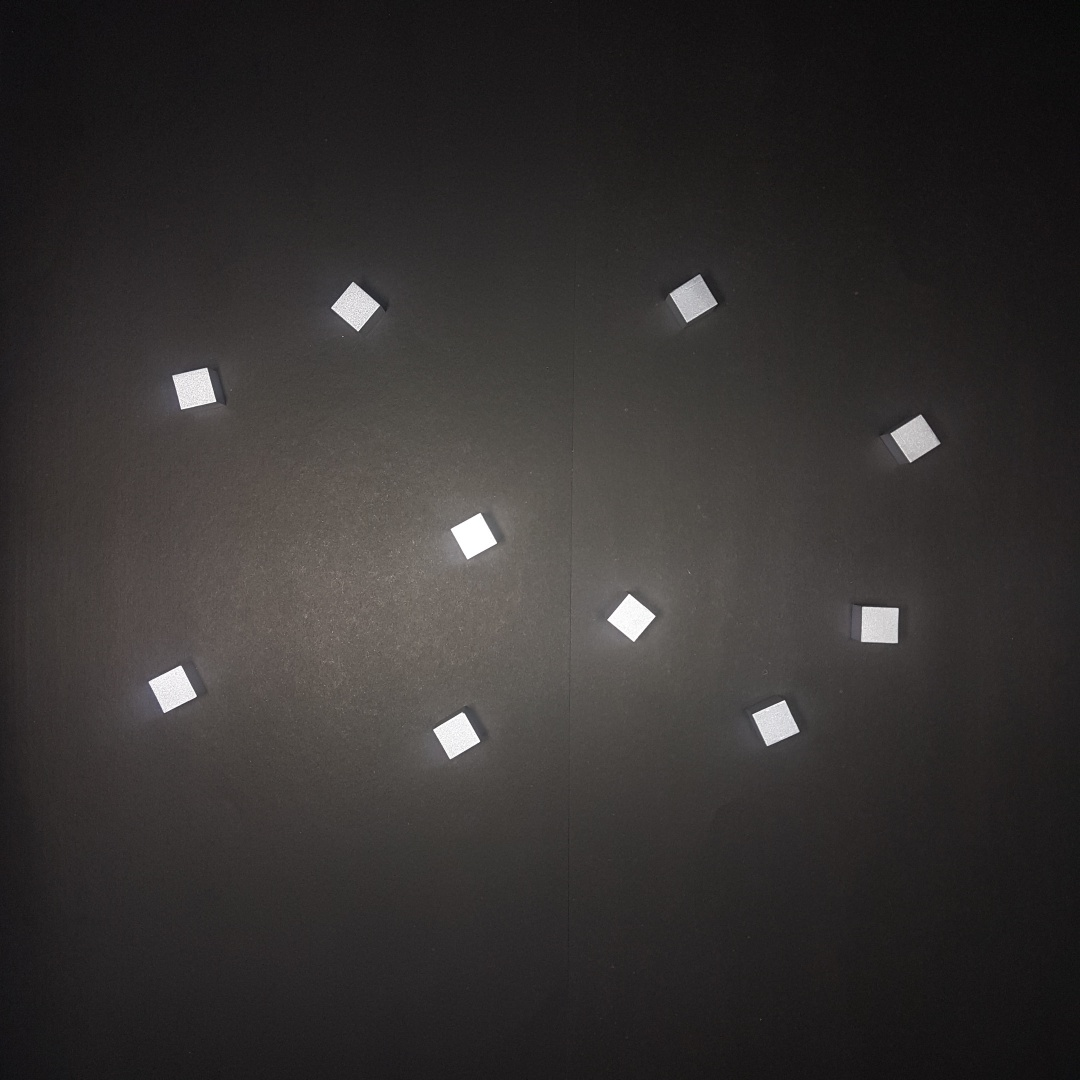
\includegraphics[width=\textwidth]{figures/202106/multiple-cubes.jpg}
         \caption{Top-view of several cubes with bright lighting from above.}
         \label{fig:multiple-cubes}
    \end{subfigure}
    \begin{subfigure}[b]{0.45\textwidth}
         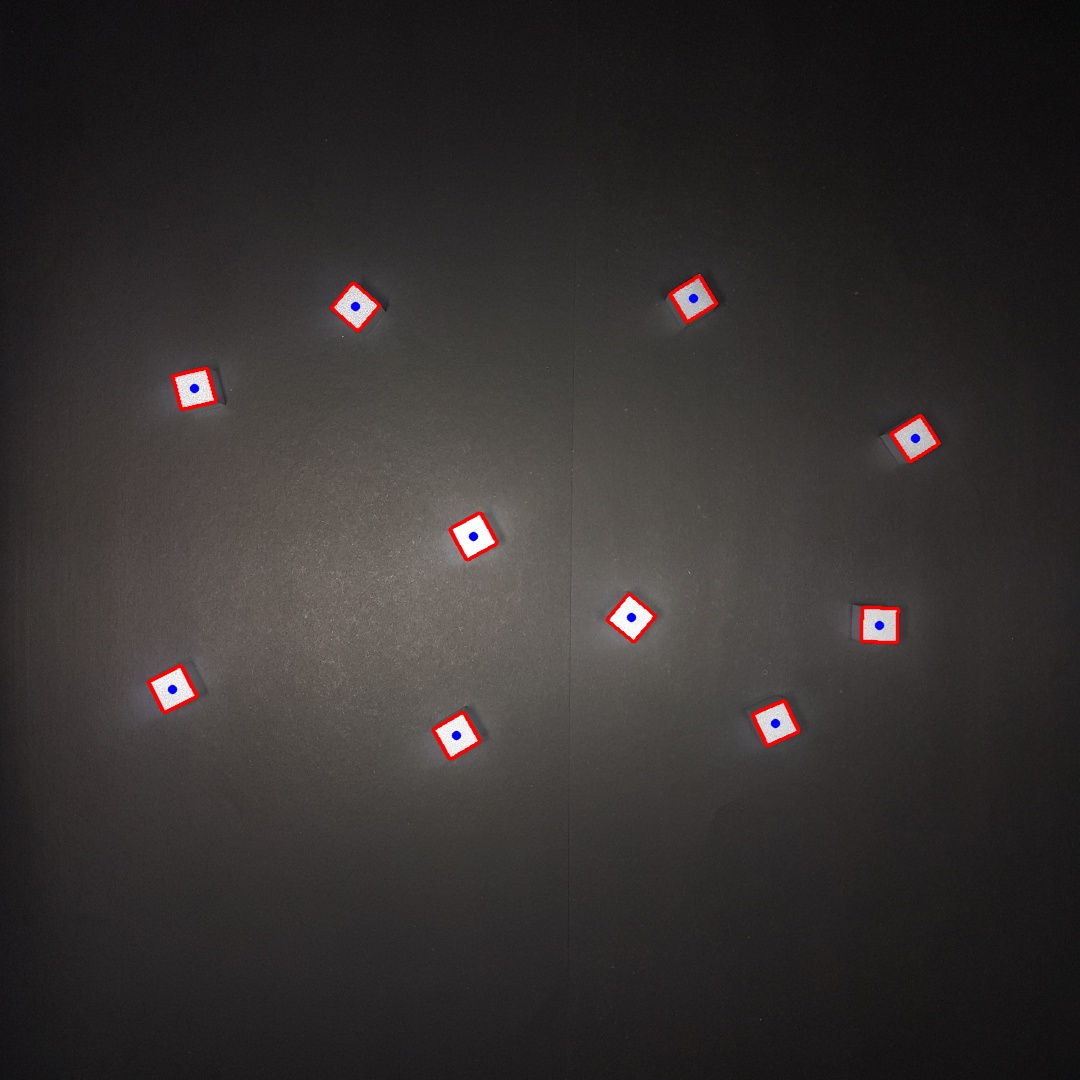
\includegraphics[width=\textwidth]{figures/202106/multiple-cube-centroids.jpg}
         \caption{Output of contour and centroid detection process for cubes in \FigRef{fig:multiple-cubes}.}
         \label{fig:multiple-cube-centroids}
    \end{subfigure}
    \captionsetup{singlelinecheck = false, justification=justified}
    \caption{Centroid detection applied to image containing multiple cubes.}
    \label{fig:multiple-cube-detection}
\end{figure}

\pendsign

\section[2021/06/16]{Thursday, 16 June 2021}

\subsection{Camera Calibration}

The next step in the development of the computer vision subsystem is the mapping of the points in the image coordinate system to coordinates in the world coordinate system. In order to perform this, several parameters about the camera and its orientation need to be known. These parameters can be divided into two categories, namely intrinsic and extrinsic parameters. Intrinsic parameters describe internal properties inherent to the camera itself and include the principal point $(c_x,c_y)$ and the focal lengths ($f_x$ and $f_y$) of the camera. Extrinsic parameters describe the location and orientation of the camera with respect to the world coordinates of the scene and include the rotation and translation transformations that need to be performed to map a point in the world coordinate system to image coordinate system. These transformations are captured by the rotation-translation matrix $[\textbf{R}|\textbf{t}]$. Camera calibration is used to estimate the intrinsic characteristics of the camera while camera localisation is used to estimate the extrinsic parameters of the camera \cite{Szeliski2010}. This description is based on the pinhole camera model which is shown in \FigRef{fig:pinhole-camera-model}.

\begin{figure}[!ht]
    \centering
    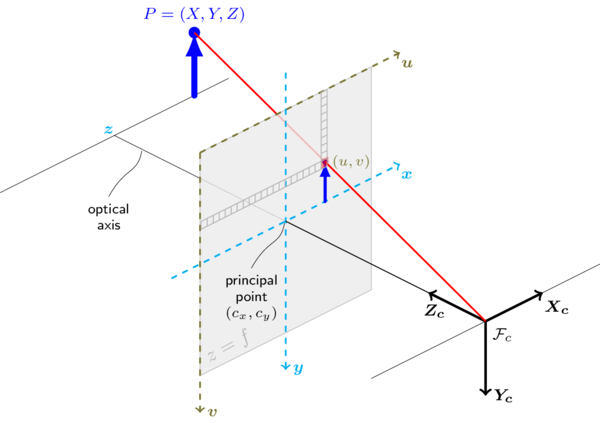
\includegraphics[width=0.7\linewidth]{figures/202106/pinhole-camera-model.png}
    \caption{Diagram showing the parameters of the pinhole camera model. Source: \cite{OpenCVCameraCalibration}}
    \label{fig:pinhole-camera-model}
\end{figure}

The intrinsic parameters of the camera can be expressed as a calibration matrix $\textbf{K}$ as shown in \EquRef{eqn:calibration-matrix} below.

\begin{equation}
    \textbf{K}=
    \begin{bmatrix}
        f_x & s & c_x \\ 
        0 & f_y & c_y \\ 
        0 & 0 & 1
    \end{bmatrix}
  \label{eqn:calibration-matrix}
\end{equation}

The parameter $s$ captures the skew of the sensor axes that occurs as a result of the optical axis not being exactly perpendicular to the sensor plane. However, for practical purposes $s$ can be set to 0. Since the extrinsic parameters are captured by the rotation-translation matrix $[\textbf{R}|\textbf{t}]$, both the intrinsic and extrinsic parameters are captured by the product of this matrix and the calibration matrix $K$. This 3 x 4 product matrix is refered to the camera matrix $P$ and is defined in \EquRef{eqn:camera-matrix} below.

\begin{equation}
    \textbf{P}=\textbf{K}[\textbf{R}|\textbf{t}]
  \label{eqn:camera-matrix}
\end{equation}

The camera matrix is sufficient to map the world coordinates to the coordinates on the image plane provided that the pinhole camera model is used and no lens distortion effects are present. This mapping is captured by \EquRef{eqn:pinhole-camera-mapping} below where $(u,v)$ represent the pixel coordinates on the image plane, $(X,Y,Z)$ represents a point in the world coordinate system and $s$ is simply a scaling factor \cite{OpenCVCameraCalibration}.

\begin{equation}
    s
    \begin{bmatrix}
        u \\ 
        v \\ 
        1
    \end{bmatrix}
    =
    \textbf{P}
    \begin{bmatrix}
        X \\ 
        Y \\ 
        Z \\
        1
    \end{bmatrix}
  \label{eqn:pinhole-camera-mapping}
\end{equation}

Therefore, in order to map the centroids of the cubes from the image coordinate space to the world coordinate space, the intrinsic and extrinsic parameters of the camera need to be determined. Furthermore, real world cameras have lens distortion effects that need to be adjusted for. The OpenCV library was used to perform this camera calibration process to produce the intrinsic parameters of the camera. Furthermore, in order to account for the lens distortion, an improved intrinsic matrix was computed. It must be noted that most literature identifies the camera matrix $P$ as a product of the intrinsic and extrinsic matrices. However, OpenCV refers to the intrinsic matrix $K$ as the camera matrix. 

\begin{figure}[H]
    \centering
    \begin{subfigure}[b]{0.45\textwidth}
         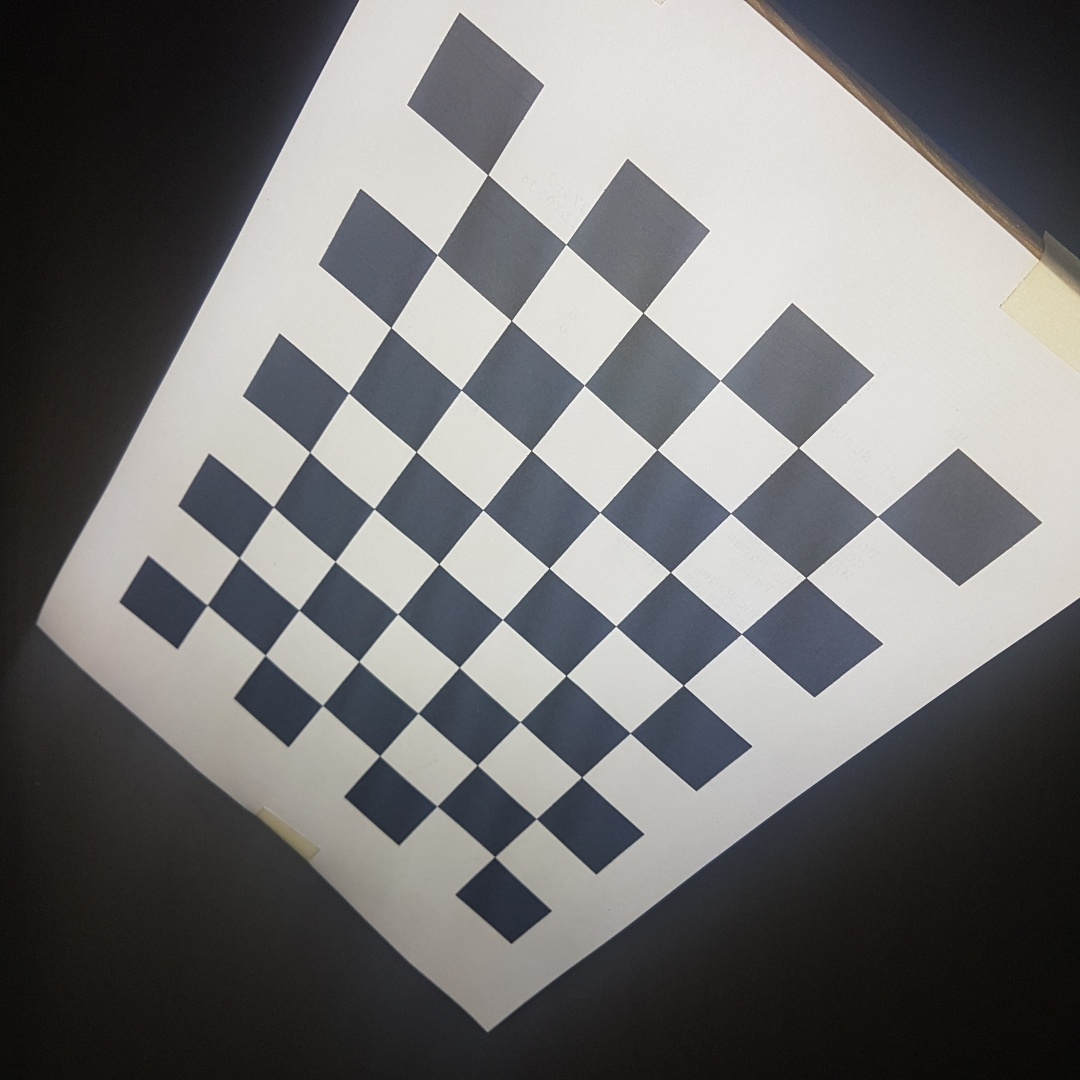
\includegraphics[width=\textwidth]{figures/202106/original-checkerboard.jpg}
         \caption{Checkerboard placed at an angle to facilitate the camera calibration process.}
         \label{fig:original-checkerboard}
    \end{subfigure}
    \begin{subfigure}[b]{0.45\textwidth}
         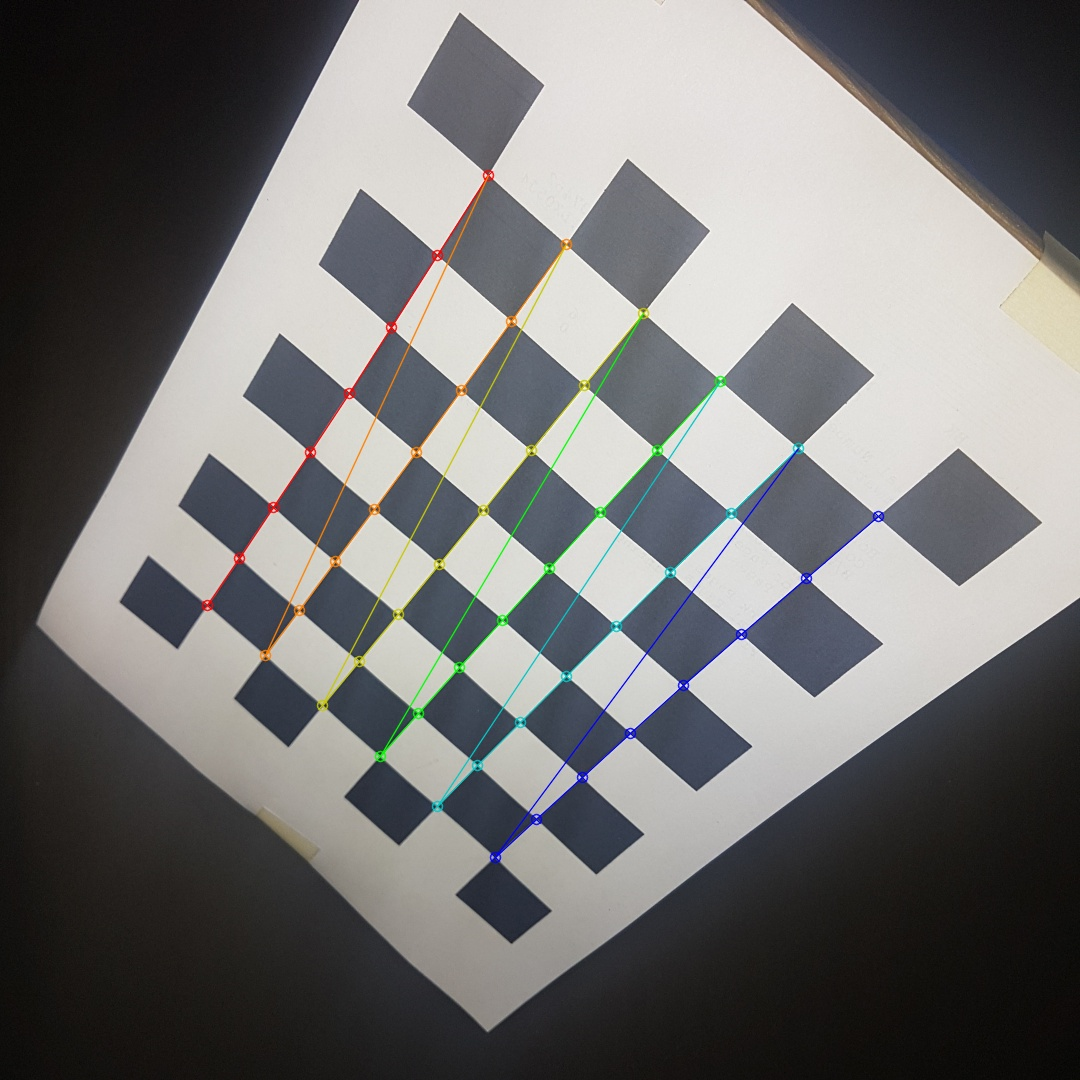
\includegraphics[width=\textwidth]{figures/202106/detected-checkerboard.jpg}
         \caption{\FigRef{fig:original-checkerboard} with various keypoints identified and highlighted.}
         \label{fig:detected-checkerboard}
    \end{subfigure}
    \captionsetup{singlelinecheck = false, justification=justified}
    \caption{Images showing the initial stages of the camera calibration process.}
    \label{fig:checkerboard-calibration}
\end{figure}

In order to perform the camera calibration process and account for the lens distortion, 35 images were taken of a 8x6 checkerboard at various positions and orientations within the camera's \ac{FOV} such as shown in \FigRef{fig:original-checkerboard}. Various known points were subsequently identified on the checkerboard as shown in \FigRef{fig:detected-checkerboard} to facilitate computation of the camera matrix. The improved camera matrix as well as the distortion coefficients describing the tangential and radial lens distortion are used to remap a distorted image as shown in \FigRef{fig:distorted-checkerboard} as to remove the distortion. The undistorted image is shown in \FigRef{fig:undistorted-checkerboard}. Note how the checkerboard lines are perfectly aligned with the red ground truth lines while they are compressed inwards in the distorted image in \FigRef{fig:distorted-checkerboard}.

\begin{figure}[H]
    \centering
    \begin{subfigure}[b]{0.45\textwidth}
        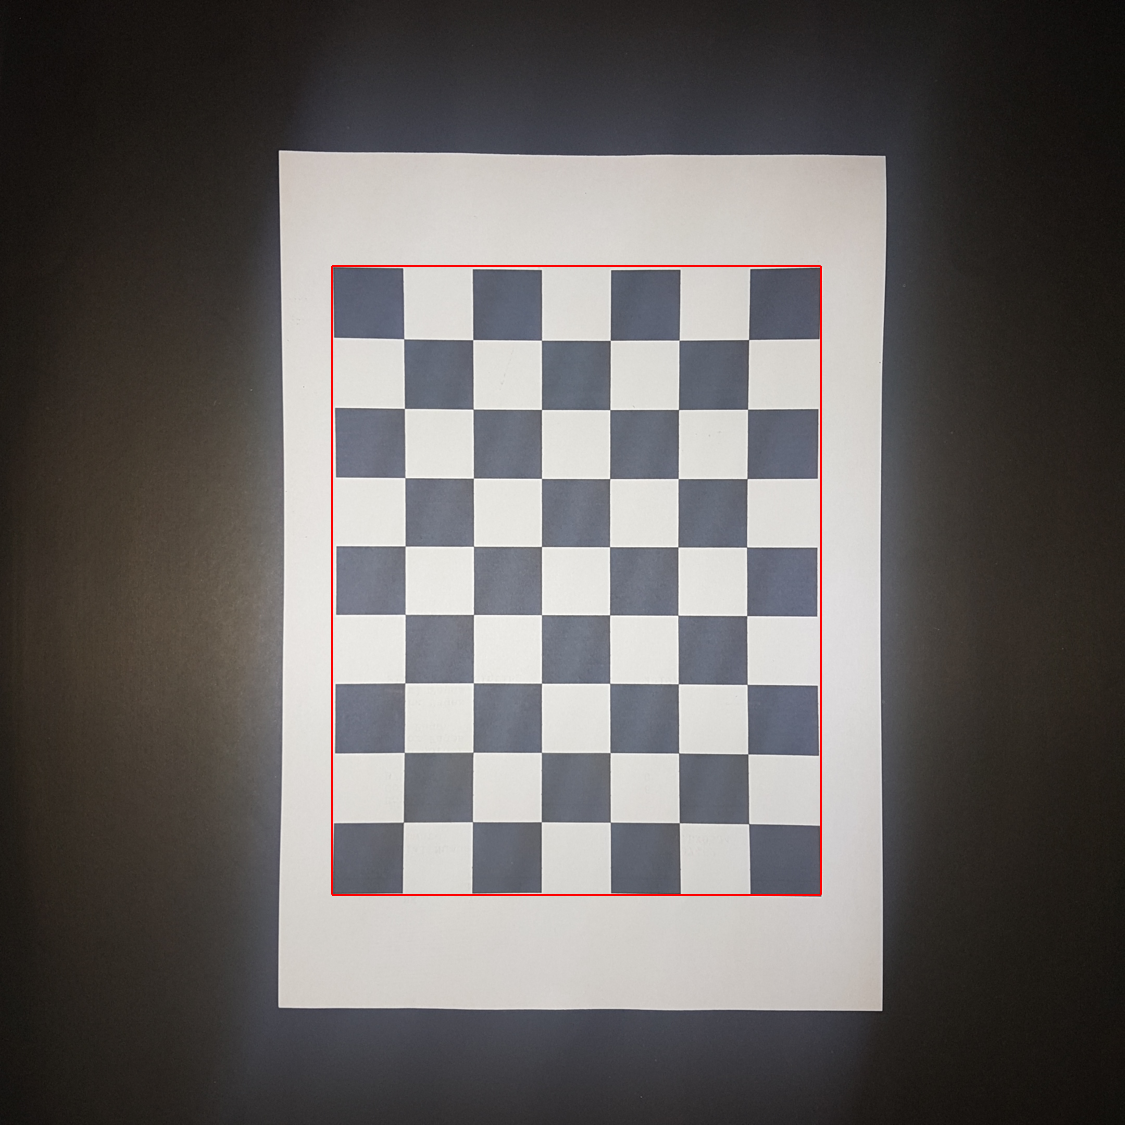
\includegraphics[width=\textwidth]{figures/202106/distorted-checkerboard.png}
        \caption{Original distorted image of the checkerboard.}
        \label{fig:distorted-checkerboard}
    \end{subfigure}
    \begin{subfigure}[b]{0.45\textwidth}
        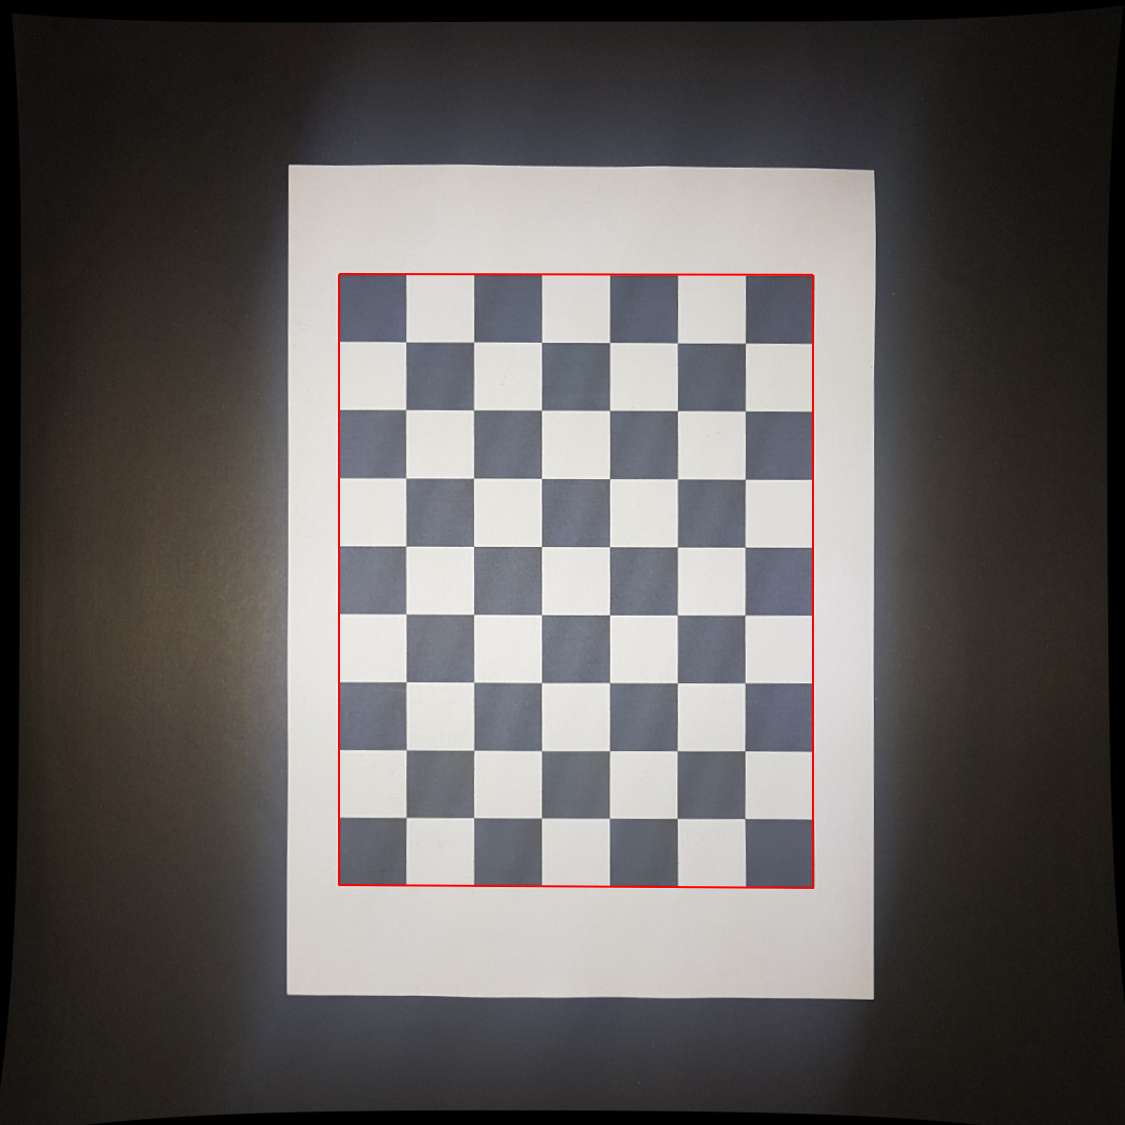
\includegraphics[width=\textwidth]{figures/202106/undistorted-checkerboard.png}
        \caption{Undistorted version of \FigRef{fig:distorted-checkerboard}}
        \label{fig:undistorted-checkerboard}
    \end{subfigure}
    \captionsetup{singlelinecheck = false, justification=justified}
    \caption{Images showing the effect of lens distortion.}
    \label{fig:checkerboard-distortion}
\end{figure}


\pendsign

\section[2021/06/29]{Wednesday, 29 June 2021}

With the machine vision component well-developed, the focus of the project moves to the mechanical design of the robot. The main components of this mechanical design involve the end-effector mechanism as well as the gantry robot required to move this mechanism throughout 3D space. Since the design of the rest of the robot relies on the design of the end-effector mechanism, this mechanism is investigated first.

\subsection{End-Effector Mechanism Design}

For the purposes of this project, the end-effector subsystem refers to the components responsible for enabling the direct manipulation of the cube. These components include the vacuum pad, tubing and vacuum generation system. The end-effector subsystem is attached to the gantry robot by means of an end-effector mechanism. In order to design this component, the machine design procedure was followed. The first step of this procedure involves understanding the requirements of the machine.

\subsubsection{Requirements}

The end-effector mechanism requirements are listed below. The end-effector mechanism should:

\begin{compactitem}
    \item Attach the end effector the the gantry robot.
    \item Maintain the suction-pad component in a vertical orientation.
    \item Allow limited linear buffered motion of the vertical suction-pad component along the z-axis w.r.t the gantry robot.
    \item The linear buffer should facilitate at least a 5mm range of linear motion.
    \item The purpose of the linear buffer is to allow the robot to target a z-axis position slightly below the intended z-axis position to ensure the cube is definitely touching the placement surface so the cube is not released in mid-air.
    \item Allow the vertical suction-pad components to rotate about the z-axis.
    \item Allow the connection of a drive mechanism to drive the rotation about the z-axis.
    \item Allow the vacuum tubing to be routed to the gantry robot.
\end{compactitem}

\subsubsection{Tolerance Investigation}

Due to my limited experience with mechanical design, it was decided perform a series of iterations of potential design solutions using Fusion 360 \ac{CAD} software. These designs were printed using the Ender 3D printer with black PLA filament. The purpose of this was to familiarise myself with \ac{CAD} software as well as identify issues that arise when converting a \ac{CAD} design into a physical realisation.

In order to begin a proof of concept design, the components that the end-effector mechanism needed to connect to from the vacuum subsystem were considered. Specifically, the end-effector mechanism needed to attach to the ZPT08UN-B5 vacuum pad adaptor which connects to the M-5AU-6 barbed pneumatic connector. The barbed connector consists of a male M5 thread which has a diameter of 5mm as well as a hexagonal wrench band with a parallel edge distance of 7mm. The first design concept explored was to design a 3D part that the barbed connector is placed into with the male thread protruding from the design for the female M5 thread of the vacuum pad adaptor to connect to. 

In order to create a 3D part that allows the barbed connector to slot into, the size of the holes and profiles for the thread and hexagonal band needed to be determined. The exact dimensions of the part could not be used as 3D printed holes are always smaller than designed due the the triangulation that takes place during mesh conversion. Therefore, a test piece was designed to test the best tolerance to use for both of these components. For the hexagonal profile, a 5mm deep section was defined in the test 3D print with 4 variations designed with 7mm, 7.2mm, 7.4mm and 7.6mm distances between the parallel lines of the hexagon. Similarly, a 1.2mm deep profile was created for the thread with 5mm, 5.2mm, 5.4mm and 5.6mm hole diameters. The tolerance testing shows that a tolerance of 0.4mm for both components provided the best fit. \FigRef{fig:pneumatic-connector-tolerances} shows the components designed and 3D printed to test the tolerances of the pneumatic connector as well as the support rings for the vacuum pad rod of \FigRef{fig:vacuum-pad-rod}.

\begin{figure}[H]
    \centering
    \begin{subfigure}[b]{0.45\textwidth}
        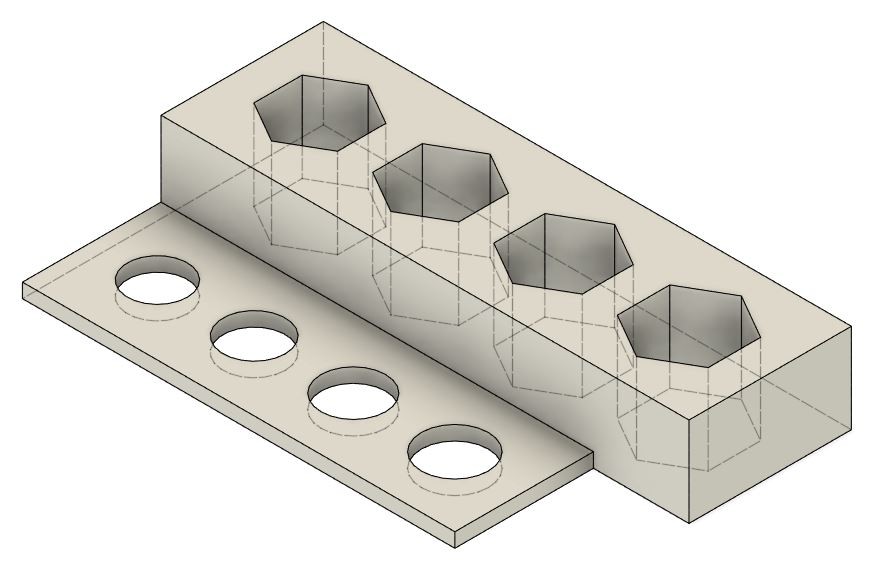
\includegraphics[width=\textwidth]{figures/202106/pneumatic-connector-tolerances.JPG}
        \caption{\ac{CAD} design of component with various hole profile sizes to test the pneumatic connector hole tolerance.}
        \label{fig:pneumatic-connector-tolerances-cad}
    \end{subfigure}
    \begin{subfigure}[b]{0.45\textwidth}
        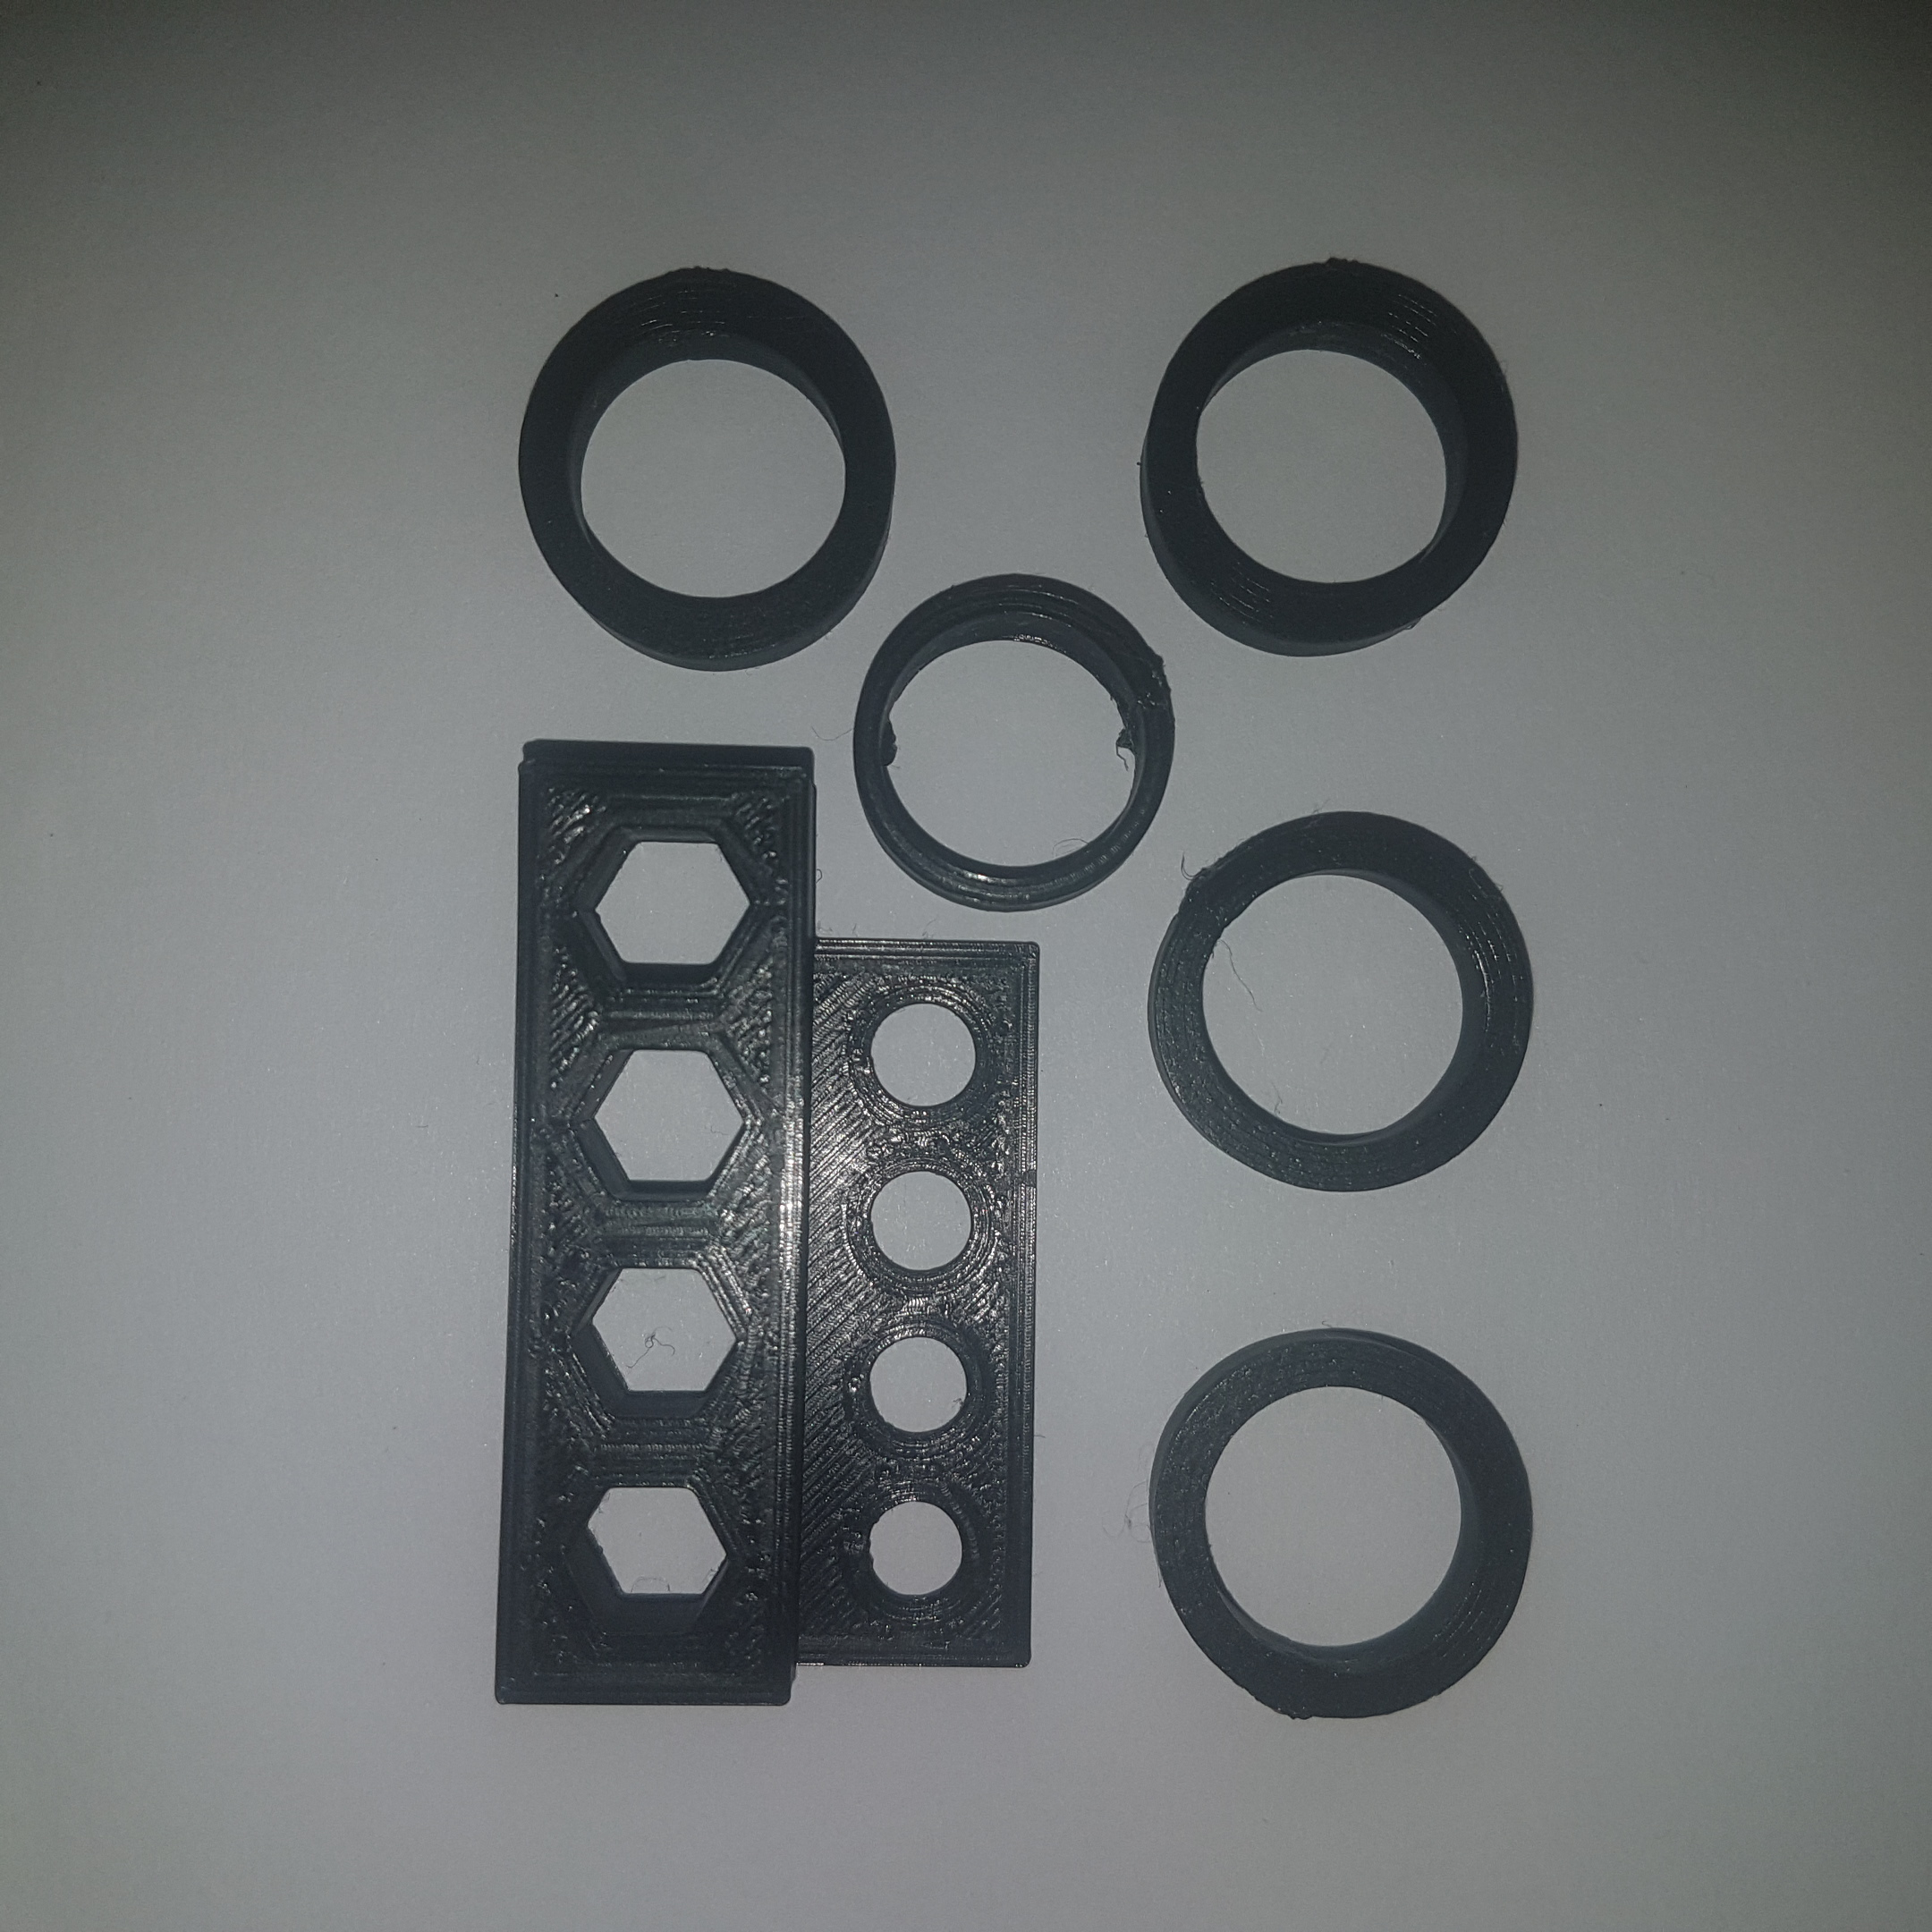
\includegraphics[width=\textwidth]{figures/202106/pneumatic-connector-tolerances-photo.jpg}
        \caption{3D print realisation of the \ac{CAD} design of \FigRef{fig:pneumatic-connector-tolerances-cad} as well as ring tolerance check components.}
        \label{fig:pneumatic-connector-tolerances-photo}
    \end{subfigure}
    \captionsetup{singlelinecheck = false, justification=justified}
    \caption{\ac{CAD} designs and corresponding physical components used to test the pneumatic connector tolerances.}
    \label{fig:pneumatic-connector-tolerances}
\end{figure}

\subsubsection{Proof of Concept Design}

The initial design investigated for the end-effector mechanism was centred around the requirement of a 5mm linear displacement buffer. A buffer can be implemented as a linear rod with guide holes as well as a ridge on the rod that allows a spring to be placed between the ridge and one of the guide holes. This provides a linear buffering action along the axis to which the rod is aligned. The design idea with respect to the end-effector mechanism is to mount the vacuum pad on the end of the rod opposite to the spring and position the rod in a vertical orientation with the vacuum pad at the bottom where it can access cubes on the plane below it. When the vacuum pad is not in contact with anything, the spring and the force of gravity push the vacuum pad into its lowest position. When a force is applied vertically upwards against the vacuum pad, as is the case when the vacuum pad is pressed against a cube, the spring will compress if the force is greater than the gravitational force on the moving rod as well as the spring force at that length.

An issue with this simple design is that the vacuum tube needs to be routed to the vacuum pad as well as the fact that the vacuum pad needs to be rotatable by an external motor. The tubing routing issue is solved by making the rod hollow and routing the tube through the rod and out top of the rod. Furthermore, it is noted that the system only needs to be able to rotate a minimum of 90 degrees to be able to realise any orientation of a cube in terms of rotation about the z-axis. The rubber tubing is comfortably able to absorb this degree of torsion and therefore, no additional mechanisms are required to route the tube.

\begin{figure}[H]
    \centering
    \begin{subfigure}[b]{0.45\textwidth}
        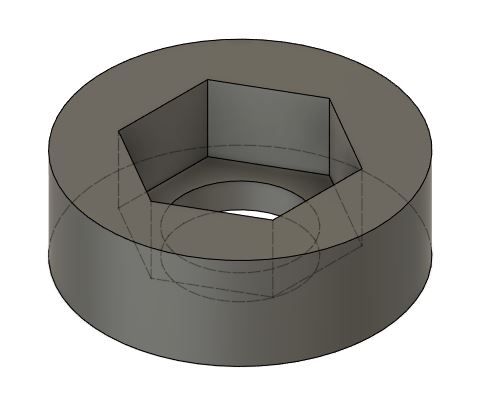
\includegraphics[width=\textwidth]{figures/202106/vacuum-pad-rod-base.JPG}
        \caption{\ac{CAD} design of the base section of the vacuum pad rod of \FigRef{fig:vacuum-pad-rod-cad}.}
        \label{fig:vacuum-pad-rod-base-cad}
    \end{subfigure}
    \begin{subfigure}[b]{0.45\textwidth}
        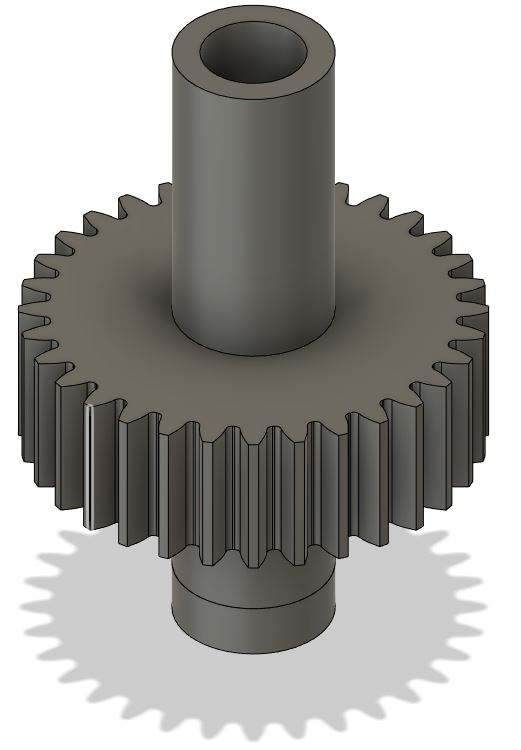
\includegraphics[width=\textwidth]{figures/202106/vacuum-pad-rod.JPG}
        \caption{\ac{CAD} design of the vacuum pad rod around which the end-effector mechanism is based.}
        \label{fig:vacuum-pad-rod-cad}
    \end{subfigure}
    \begin{subfigure}[b]{0.45\textwidth}
        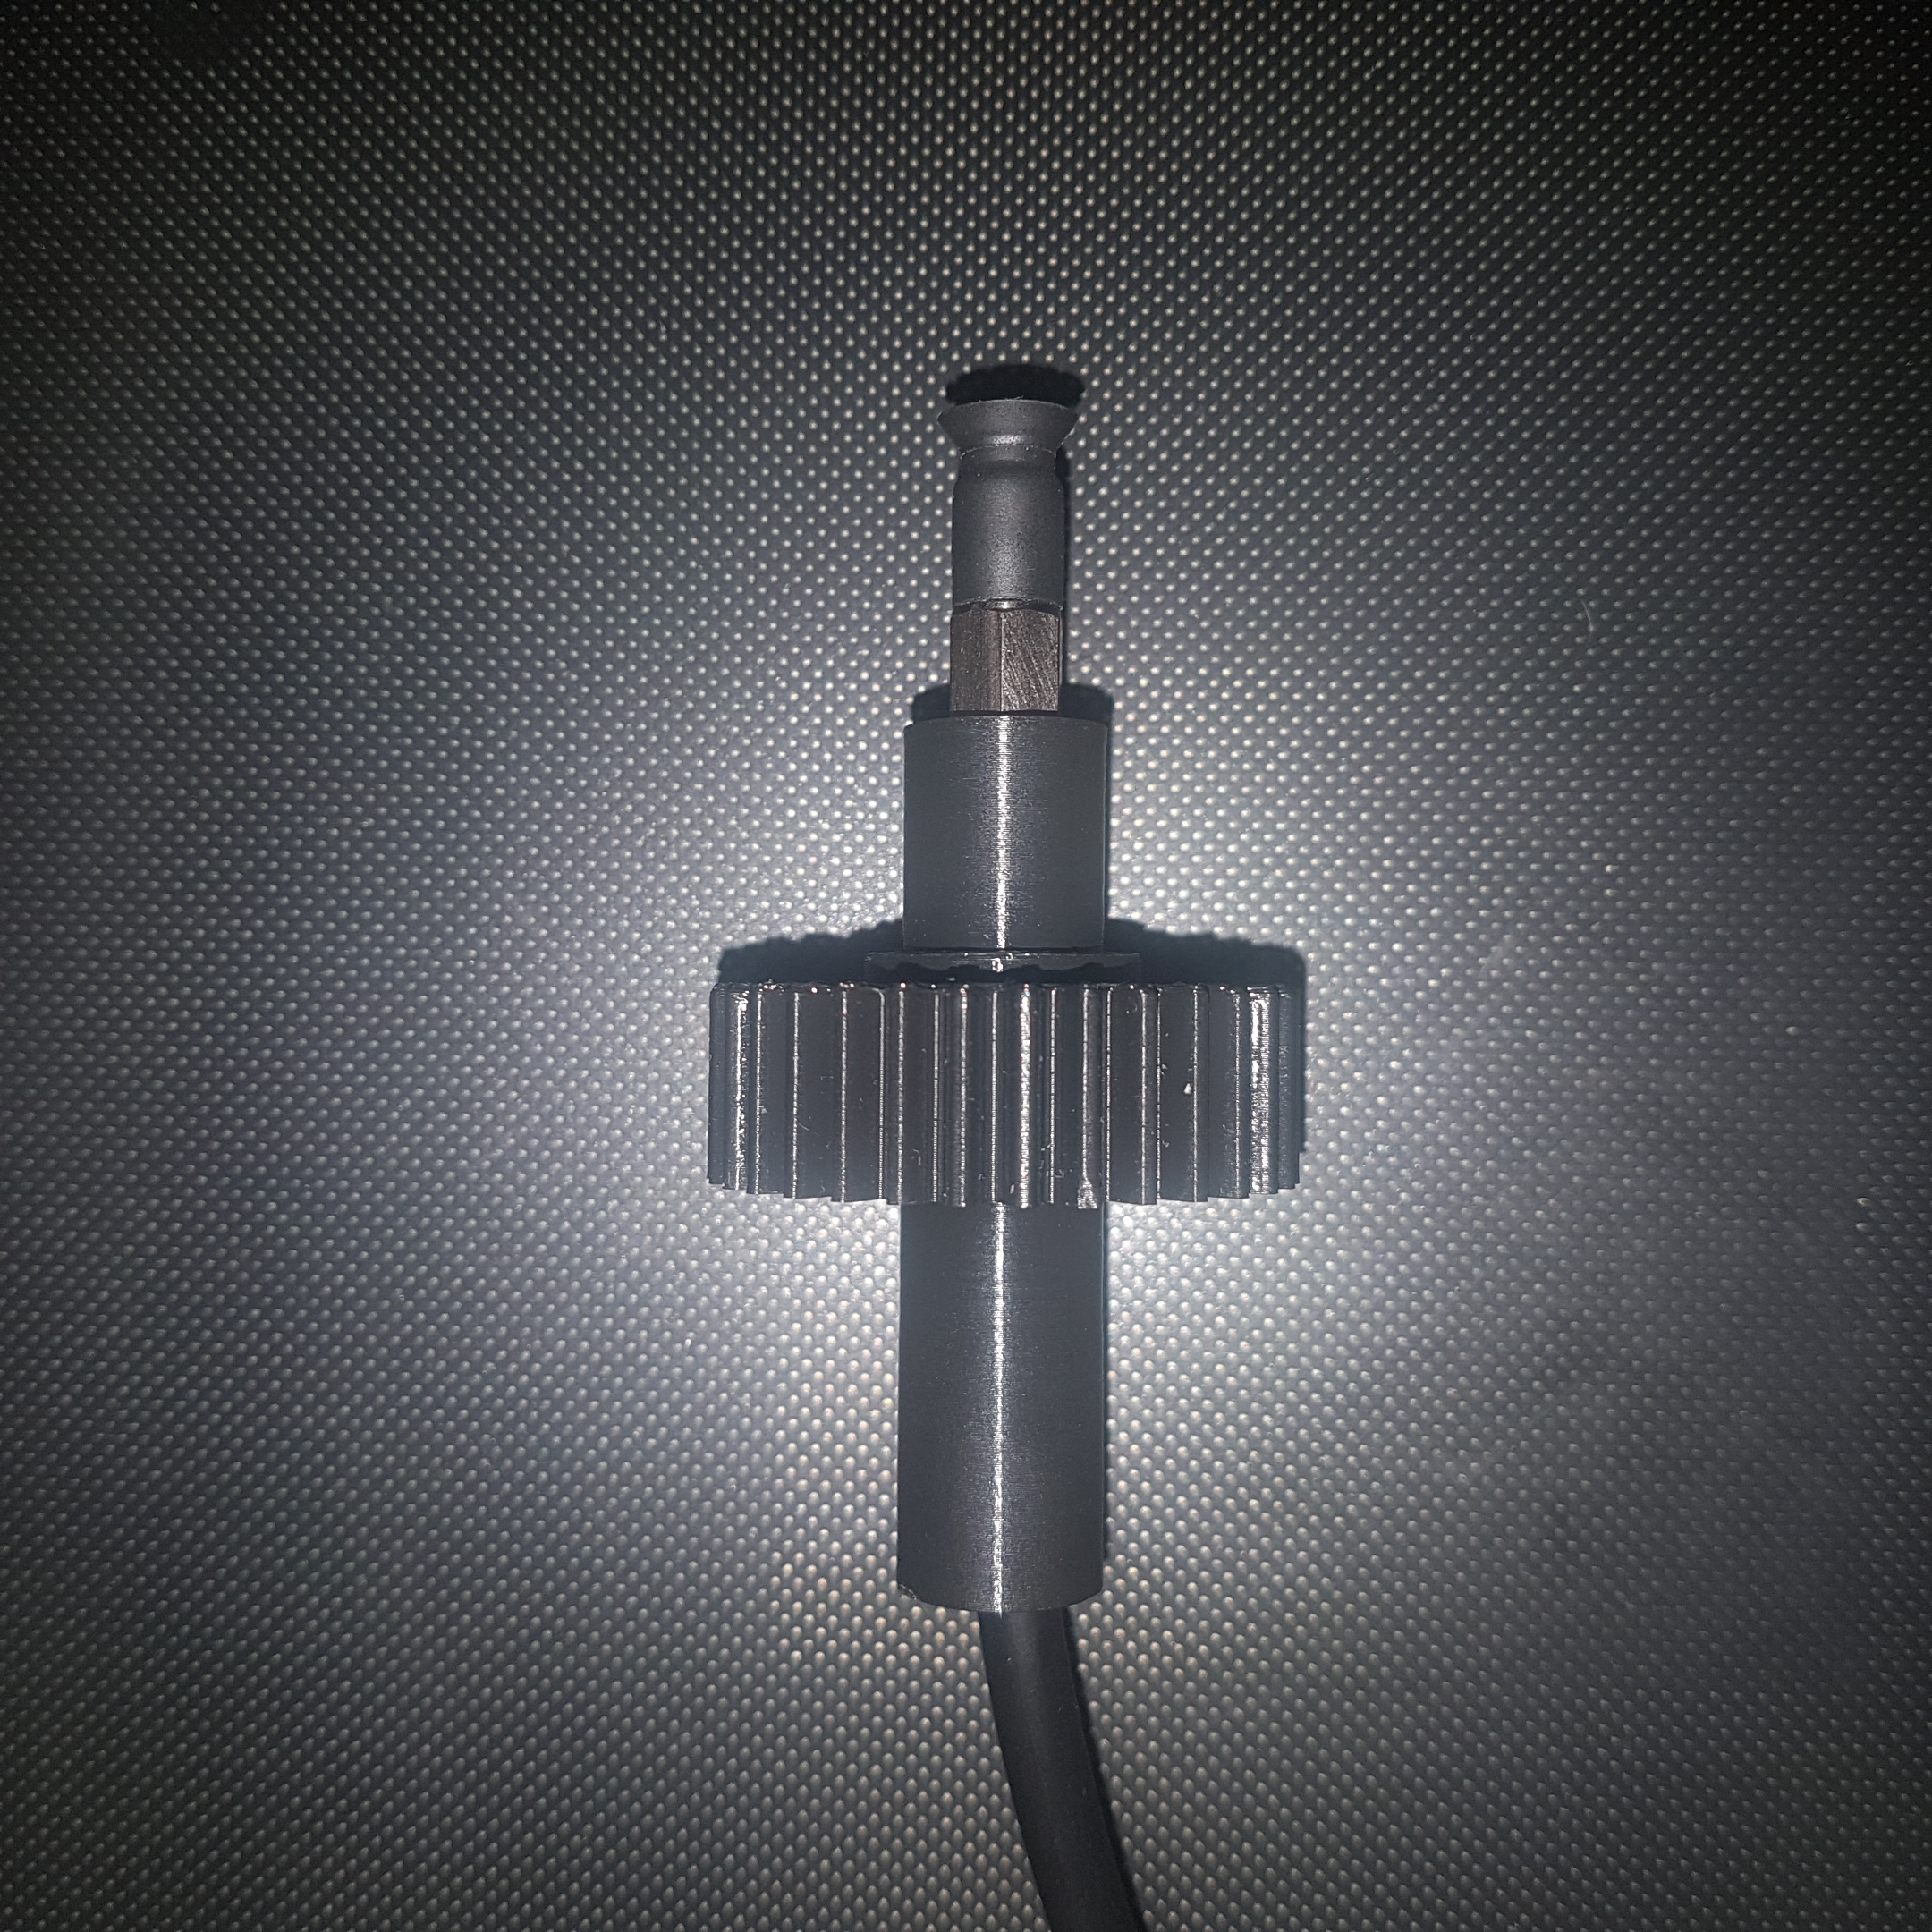
\includegraphics[width=\textwidth]{figures/202106/vacuum-pad-rod-photo-side.jpg}
        \caption{Side view of the 3D printed realisation of the vacuum pad rod of \FigRef{fig:vacuum-pad-rod-cad}}
        \label{fig:vacuum-pad-rod-photo-side}
    \end{subfigure}
    \begin{subfigure}[b]{0.45\textwidth}
        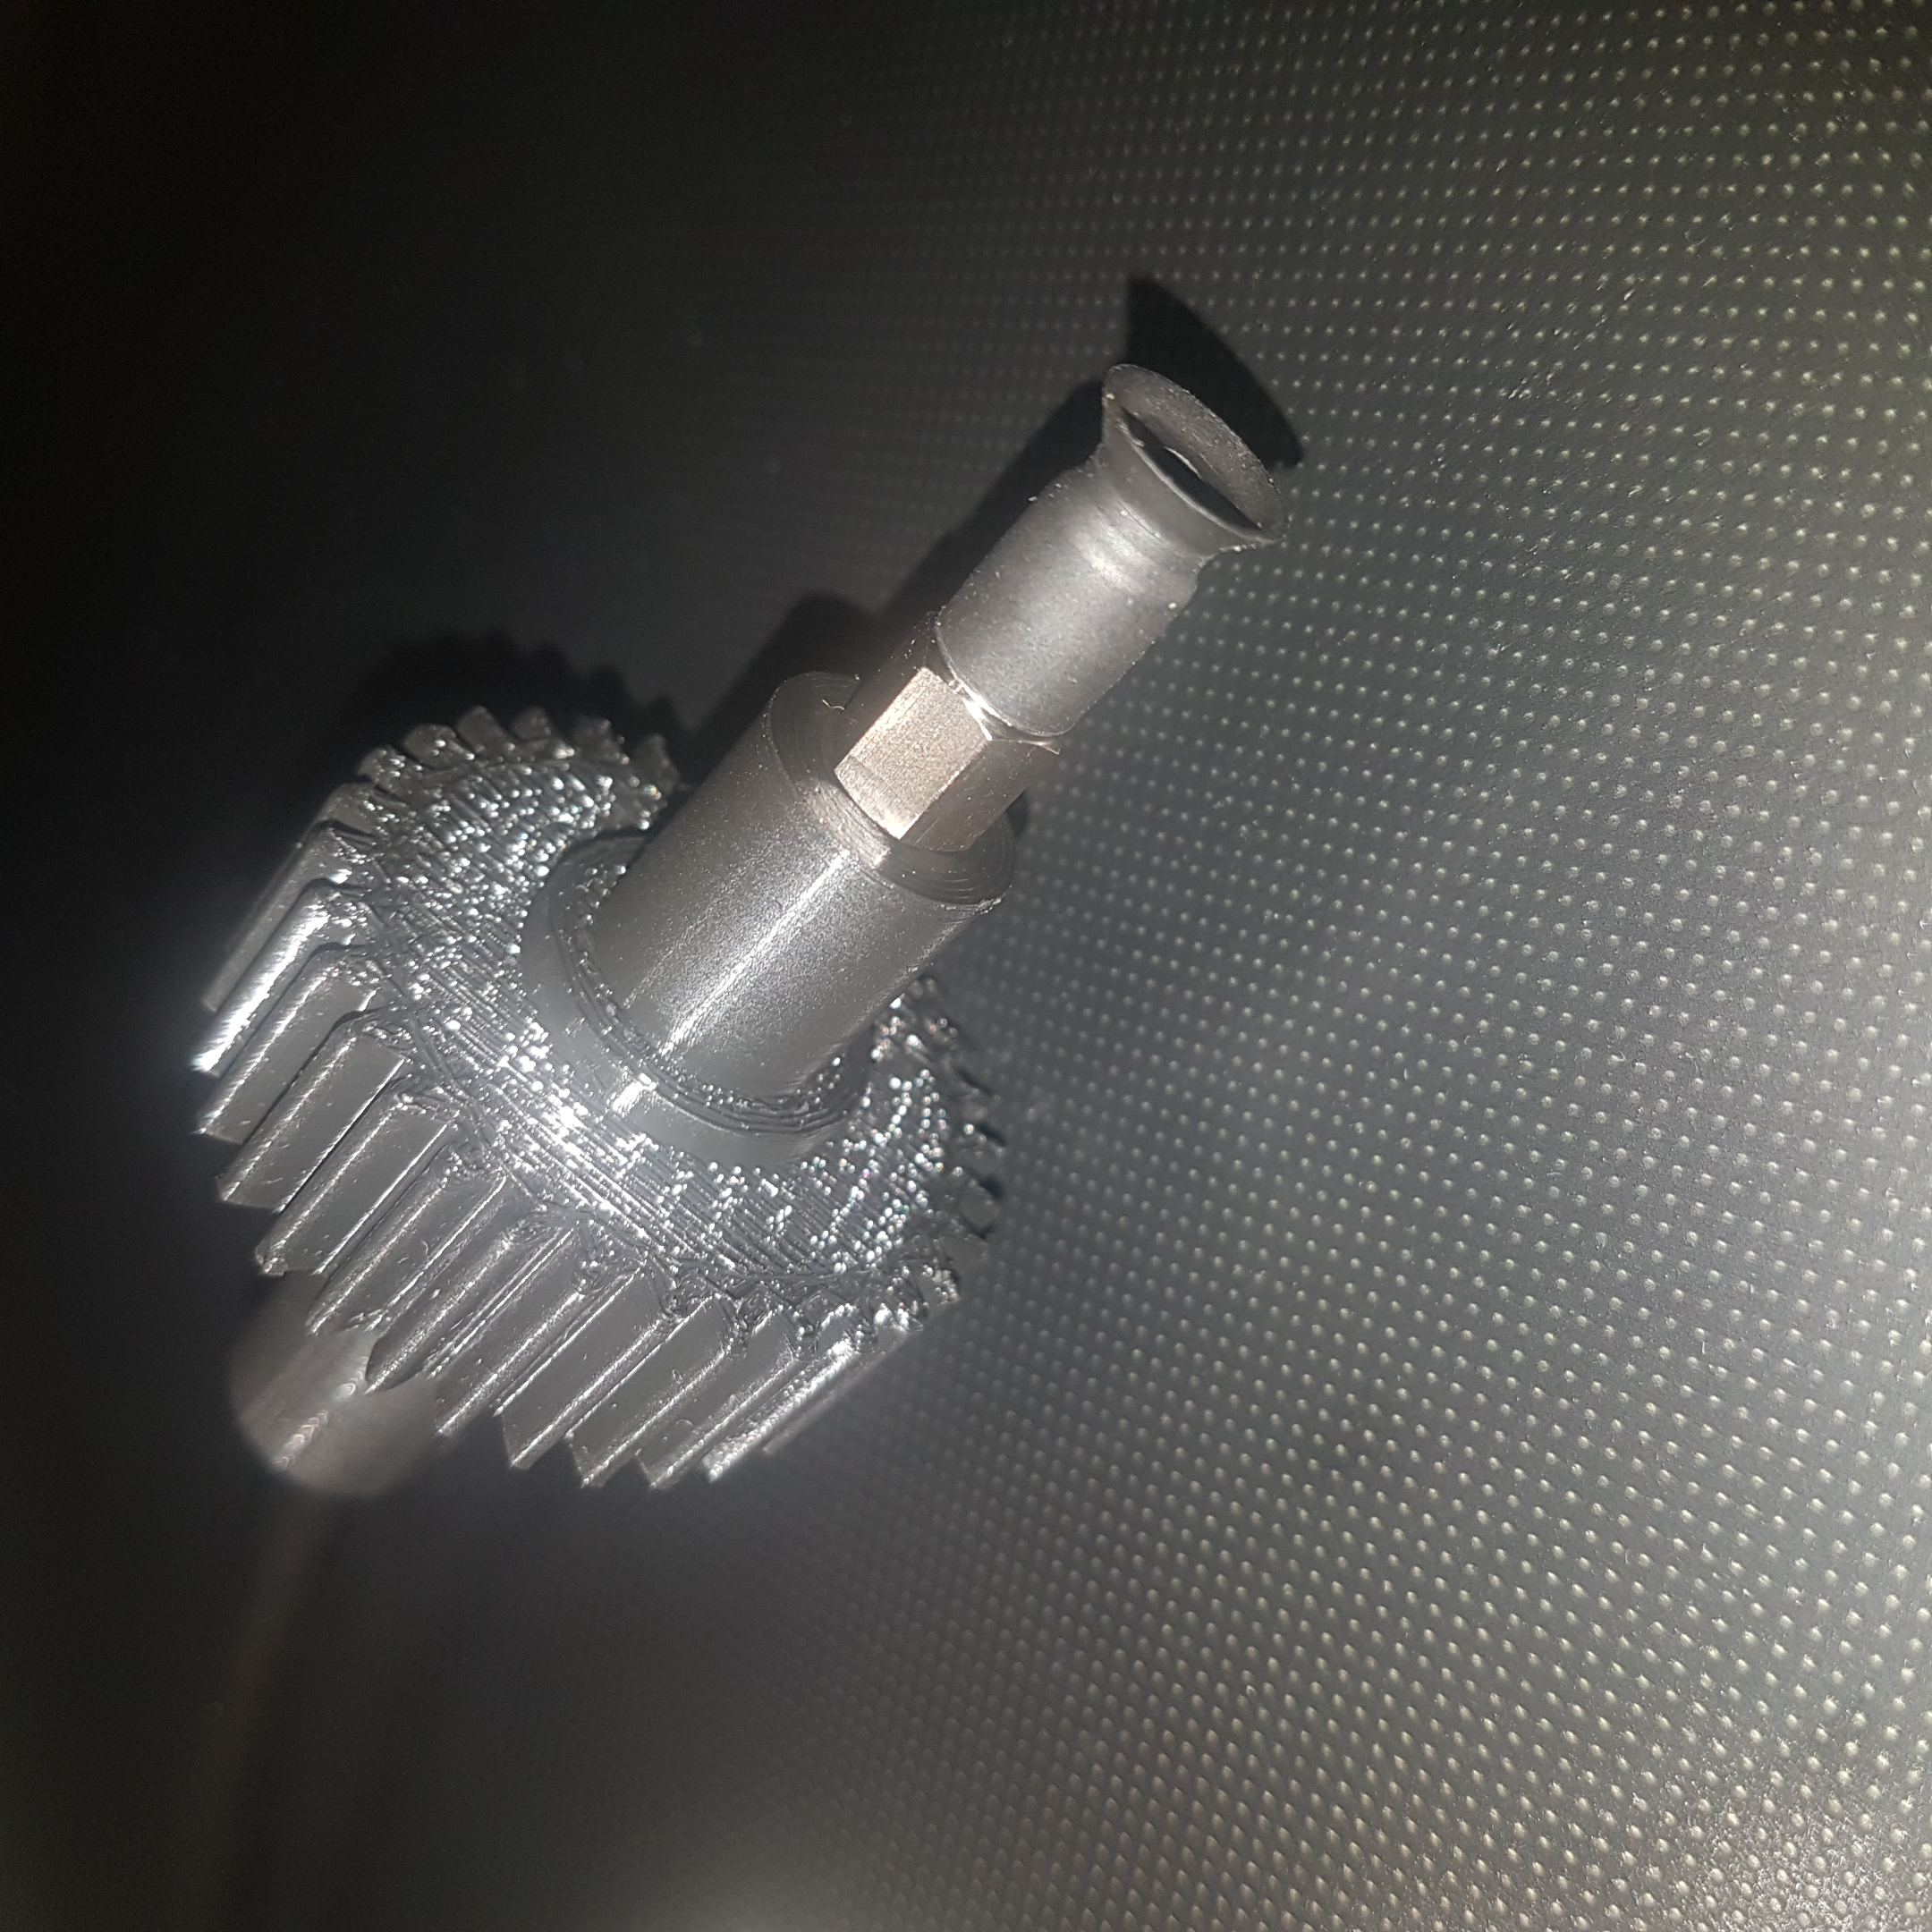
\includegraphics[width=\textwidth]{figures/202106/vacuum-pad-rod-photo-angle.jpg}
        \caption{Angled view of the 3D printed realisation of the vacuum pad rod of \FigRef{fig:vacuum-pad-rod-cad}}
        \label{fig:vacuum-pad-rod-photo-angle}
    \end{subfigure}
    \captionsetup{singlelinecheck = false, justification=justified}
    \caption{CAD design and corresponding physical realisation of the vacuum pad rod in the end-effector mechanism.}
    \label{fig:vacuum-pad-rod}
\end{figure}

The second design consideration is how the rod will be rotated to rotate the vacuum pad given that the rod has linear motion of 5mm. The design solution to this investigated in the proof of concept design is the use of a gear attached to the rod which can be driven by a motor gear. The use of gears with their axes aligned with the rod axis allows the linear motion to be absorbed by the linear freedom of movement between the gear teeth. In order to absorb this motion, the height of the gear attached to the rod needs to be at least 5mm greater than the height of the motor gear is the maximum overlap is to be always maintained assuming the position of the motor is fixed with respect to the component supporting the rod. An alternative design that could be explored in the future, is fixing the linear position of the motor with respect to the spring to reduce the gear height and using the weight of the motor to act in a similar manner to the spring force. \FigRef{fig:vacuum-pad-rod} shows the CAD designs developed for the vacuum pad rod as well as the corresponding 3D printed prototypes.

\pendsign